\documentclass[10pt]{article}

%==============================
% Document Metadata
%============================== 
\usepackage[pdftex,
    pdfauthor={Rukmal Weerawarana},
    pdftitle={Homework 1 Solutions - FE 621},
    pdfsubject={FE 621 - Computational Methods in Finance}
]{hyperref}


%==============================
% Package Imports
%==============================    
\usepackage[ruled]{algorithm2e} % typeset algorithms
\usepackage[authordate, maxcitenames=1]{biblatex-chicago} % chicago bibliography style
\usepackage{amsmath} % math environment stuff
\usepackage{amssymb} % additional math symbols
\usepackage[toc, page]{appendix} % Appendix referencing
\usepackage{booktabs} % Table lines
\usepackage{comment} % enables the use of multi-line comments (\ifx \fi)
\usepackage[skip=5pt, labelfont=bf]{caption} % caption formatting
\usepackage{csvsimple} % CSV import to Table
\usepackage{fancyhdr} % Header
\usepackage{fancyvrb} % Verbatim text
\usepackage{float} % Controlling figure border
\usepackage[headings]{fullpage} % Set all margins to 1.5 cm
\usepackage{graphicx} % Figures
\usepackage{listings} % code embedding
\usepackage{longtable} % Multipage tables
\usepackage{pmboxdraw} % Box characters for file tree
\usepackage[dvipsnames]{xcolor} % colors for code


%==============================
% Configuration
%==============================

% Figure outline configuration
% \floatstyle{boxed}
% \restylefloat{figure}

% Bibliography configuration

\addbibresource{../bibliography.bib}

% Remapping bibliography underscores (_) and tildes (~) because Mendeley has weird exporting
% Solution from: https://tex.stackexchange.com/questions/309980/parsing-underscores-in-urls-from-mendeley

\DeclareSourcemap{ % Used when .bib/Bibliography is compiled, not when document is
    \maps{
        \map{ % Replaces '{\_}', '{_}' or '\_' with just '_'
            \step[fieldsource=url,
                  match=\regexp{\{\\\_\}|\{\_\}|\\\_},
                  replace=\regexp{\_}]
        }
        \map{ % Replaces '{'$\sim$'}', '$\sim$' or '{~}' with just '~'
            \step[fieldsource=url,
                  match=\regexp{\{\$\\sim\$\}|\{\~\}|\$\\sim\$},
                  replace=\regexp{\~}]
        }
    }
}

% Code display configuration

\newcommand*\lstinputpath[1]{\lstset{inputpath=#1}} % Setting path
\lstset{
	language=Python,
	basicstyle=\footnotesize\ttfamily,
	commentstyle=\ttfamily\color{purple!40!black},
	identifierstyle=\color{blue},
	keywordstyle=\color{ForestGreen},
	numbers=left,
	numberstyle=\ttfamily\color{gray}\footnotesize,
	stepnumber=1,
	numbersep=5pt,
	backgroundcolor=\color{white},
	showspaces=false,
	showstringspaces=false,
	showtabs=false,
	frame=single,
	tabsize=2,
	captionpos=b,
	breaklines=true,
	breakatwhitespace=false,
	title=\lstname
}
\lstset{
	language=R,
	basicstyle=\footnotesize\ttfamily,
	commentstyle=\ttfamily\color{purple!40!black},
	identifierstyle=\color{blue},
	keywordstyle=\color{ForestGreen},
	numbers=left,
	numberstyle=\ttfamily\color{gray}\footnotesize,
	stepnumber=1,
	numbersep=5pt,
	backgroundcolor=\color{white},
	showspaces=false,
	showstringspaces=false,
	showtabs=false,
	frame=single,
	tabsize=2,
	captionpos=b,
	breaklines=true,
	breakatwhitespace=false,
	title=\lstname
}

% Header and Footer configuration

\pagestyle{fancy} % set page style
\fancyhead{} % override header
\fancyfoot{} % override footer
\renewcommand{\headrulewidth}{.4pt} % set header rule width 
\renewcommand{\footrulewidth}{.4pt} % set footer rule width 
\lhead{Homework Assignment 1} % set left header
\rhead{Rukmal Weerawarana} % set right header
\lfoot{\textit{FE 621}: Computational Methods in Finance} % set left footer
\rfoot{Page \thepage} % set right footer


%==============================
% Document Content
%==============================

\begin{document}

\thispagestyle{plain}

%==============================
% Document Title
%==============================

\noindent
\large\textbf{Homework Assignment 1} \hfill \textbf{Rukmal Weerawarana} \\
\normalsize \textit{FE 621}: Computational Methods in Finance \hfill \textit{rweerawa@stevens.edu} $\mid$ 104-307-27 \\
\textit{Instructor}: Ionut Florescu \hfill Department of Financial Engineering \\
2/20/2019 \hfill Stevens Institute of Technology

\noindent\rule{\linewidth}{.1em}


%==============================
% Overview
%==============================

\section*{Overview}

In this Homework Assignment, we explore various numerical optimization methods through the lens of the Black-Scholes-Merton Option pricing model\footnote{\cite{Shreve2004}}. Using this, we calculate and explore the implied volatility of options for various assets traded on the market. Furthermore, we also explore numeric methods of differential calculation to compute the Greeks of these candidate options. Finally, we explore numeric integration and the behavior of various quadrature methods.

Unless otherwise stated, the following shorthand notation is used to distinguish between dates:

\begin{itemize}
    \item \textbf{DATA1} - Wednesday, February 6 2019 (\textit{2/6/19})
    \item \textbf{DATA2} - Thursday, February 7 2019 (\textit{2/7/19})
\end{itemize}

The content of this Homework Assignment is divided into three sections; the first discusses data gathering, formatting, and a discussion of the assets being examined. The second contains data analysis, and an exploration of implied volatility through the Black-Scholes-Merton pricing framework and related computations. Finally, the third section discusses numerical integration and the convergence of various quadrature rules.

\begin{center}
    \textit{See Appendix~\ref{appendix:source} for specific question implementations, and the project GitHub repository\footnote{\cite{Weerawarana2019}} for full source code of the {\normalfont \texttt{fe621}} Python package.}
\end{center}


%==============================
% Section 1
%==============================

\newpage

\section{Data Overview}

    \subsection{Asset Descriptions}

        \subsubsection[\textit{SPY} - SPDR S\&P 500 ETF]{\textit{SPY} - SPDR S\&P 500 ETF\footnote{\cite{StateStreetGlobalAdvisors2019}}}
        % Note: Heading is weird here because of footnote. See: https://texfaq.org/FAQ-ftnsect

        The S\&P 500 (i.e. \textit{Standard \& Poor's 500}) is a stock market index tracking the 500 largest companies on the American Stock Exchange by Market Capitalization. In this case, the market capitalization is defined as the number of outstanding shares, multiplied by the current share price. A stock market index is designed to be a metric that can be used by market observers as a benchmark to gauge the relative health of the stock market, by analyzing the aggregate performance of its largest components.
            
        However, this index is not the same as the \textit{SPY} ETF. An ETF (\textit{Exchange Traded Fund}) is a basket of stocks that is designed to track a specific index or benchmark. That is, it provides investors with exposure to a index or benchmark, without having to own all of the underlying assets that constitute a composite ETF. In addition to higher liquidity, this type of investment also provides lower transaction costs and required minimum investment to gain exposure to a given index or benchmark. It is traded on an exchange, akin to a typical traded asset.

        \subsubsection[\textit{VIX} - CBOE Volatility Index]{\textit{VIX} - CBOE Volatility Index\footnote{\cite{CBOEChicagoBoardOptionsExchange2019}}}

        The CBOE (\textit{Chicago Board Options Exchange}) volatility index, \textit{VIX} is an exchange traded product (\textit{ETP}) designed to give investors exposure to the market's expectation of 30-day volatility. It is priced using a large set of implied volatility of put and call options on the S\&P 500 index to gauge investor sentiment. Typically, the price of the VIX has an inverse relationship to the price of the S\&P 500 index. Similar to an ETF, an ETP is also traded on an exchange as a typical traded asset.


    \subsection{Data Gathering}

    For the assignment, we downloaded monthly options on \textit{Amazon Inc.} (ticker: AMZN) and \textit{S\&P 500 ETF} (ticker: SPY) at various strike prices for the following dates:
    
    \begin{itemize}
        \item \textit{02/15/19} - Friday, February 15 2019;
        \item \textit{03/15/19} - Friday, March 15 2019;
        \item \textit{04/18/19} - Thursday, April 18 2019.
    \end{itemize}

    A wide variety of option strike prices were considered, with the following ranges:
    
    \begin{itemize}
        \item \textit{AMZN} - \$1555 to \$1725 in increments of \$5 (35 strike prices);
        \item \textit{SPY} - \$256 to \$284 in increments of \$1 (29 strike prices).
    \end{itemize}

    Intra-day minute closing price data was gathered for both put and call options with expiration dates and strike prices detailed above. This intra-day data was gathered for the trading day \textit{2/6/19} (February 6 2019; \textbf{DATA1}). Additionally, intra-day minute closing price data was also downloaded for each of the underlying assets. This data was downloaded for both \textit{2/6/19} (February 6 2019; \textbf{DATA1}), and \textit{2/7/19} (February 7 2019; \textbf{DATA2}).

    This data detailed above was gathered utilizing \textit{Rblpapi}\footnote{\cite{Armstrong2018}}, which provides an R interface to data on the Bloomberg Terminal\footnote{\cite{BloombergL.P.2019}}. The data download was automated, and corresponding intra-day prices for each of the options were output to individual files. The source code for this implementation is available in Appendix~\ref{appendix:source:q1:bloomberg}.

    Furthermore, as a proxy for the \textit{risk-free rate}, we chose to utilize the effective Federal Funds Rate (FFR). This is the interest rate at which depository institutions in the United States lend reserve balances to other depository institutions overnight. This data was gathered for both dates, and correspond to \textbf{DATA1} and \textbf{DATA2}. The effective FFR is published daily by the US Federal Reserve Board of Governors, and are expressed as yields per annum.\footnote{\cite{BoardofGovernorsoftheFederalReserveSystem2019}}

        \subsubsection{Data Cleaning}

            For easier programmatic access, the data was placed in a hierarchical structure, corresponding to the \textbf{DATA1}, \textbf{DATA2} data division. Each of the option and asset prices for the corresponding days were placed in the requisite sub-folders. This directory structure is reproduced below.

            \VerbatimInput{bin/data_tree.txt}

            Option price filenames were changed to OOC format option names, discussed further below. This was done utilizing a cleaning script, written in Python. This script employs utility functions from the \texttt{fe621} Python package\footnote{\cite{Weerawarana2019}}.
    
        \subsection{Option Naming Convention}

        A modern convention for naming option contracts was proposed by the Options Clearing Commission (OCC) in 2008\footnote{\cite{OptionsSymbologyInitiative2008}}, and adopted in 2010. The OCC is an organization that acts as both the issuer and guarantor for option and future contracts. The OCC is governed by the Securities and Exchange Commission (SEC) and the Commodities Futures Trading Commission (CFTC). The current convention for option naming is best explained by example.
        
        Consider the option code, \textit{AMZN190215C01960000}. This corresponds to a \textbf{Call Option} on \textbf{Amazon Inc. (AMZN)}, with a strike price of \textbf{\$1960.00} and an expiration date of \textbf{2/15/19} (February 15 2019).
        
        The methodology of this nomenclature is explained in detail below:
    
        % Note: The number here denotes the "priority" of the pagebreak. It can range from 0-4, with 4 being highest priority (i.e. right now), and 0 being the lowest.
        \pagebreak[3]

        \begin{center}
            \textbf{\textcolor{red}{AMZN}\textcolor{MidnightBlue}{19}\textcolor{Bittersweet}{02}\textcolor{YellowOrange}{15}\textcolor{RoyalPurple}{C}\textcolor{ForestGreen}{01960}\textcolor{violet}{000}}
        \end{center}
    
        \begin{itemize}
            \item \textbf{\textcolor{red}{AMZN}} - Ticker of the company (arbitrary length; always first sequence of characters)
            \item \textbf{\textcolor{MidnightBlue}{19}} - Expiration year of the contract (shortened to two digits, i.e. 2019 $\rightarrow$ 19)
            \item \textbf{\textcolor{Bittersweet}{02}} - Expiration month of the contract
            \item \textbf{\textcolor{YellowOrange}{15}} - Expiration day of the contract
            \item \textbf{\textcolor{RoyalPurple}{C}} - Type of option (\textit{C} for call, \textit{P} for put)
            \item \textbf{\textcolor{ForestGreen}{01960}} - Dollar component of strike price (in \$; always 5 digits)
            \item \textbf{\textcolor{violet}{000}} - ${\frac{1}{1000}}^\text{th}$ Dollar component of strike price (in $\frac{1}{1000}$\$; always 3 digits)
        \end{itemize}
    
        Similarly, the following option code corresponds to a \textbf{Put Option} on \textbf{SPDR S\&P 500 ETF (SPY)}, with a strike price of \textbf{\$287.50} and an expiration date of \textbf{3/15/19} (March 15 2019):
    
        \begin{center}
            \textbf{\textcolor{red}{SPY}\textcolor{MidnightBlue}{19}\textcolor{Bittersweet}{03}\textcolor{YellowOrange}{15}\textcolor{RoyalPurple}{P}\textcolor{ForestGreen}{00287}\textcolor{violet}{500}}
        \end{center}
    
        Finally, the following option code corresponds to a \textbf{Call Option} on \textbf{CBOE Volatility Index (VIX)}, with a strike price of \textbf{\$16.35} and an expiration date of \textbf{4/18/19} (February 18 2019):
    
        \begin{center}
            \textbf{\textcolor{red}{VIX}\textcolor{MidnightBlue}{19}\textcolor{Bittersweet}{04}\textcolor{YellowOrange}{18}\textcolor{RoyalPurple}{C}\textcolor{ForestGreen}{00016}\textcolor{violet}{350}}
        \end{center}


%==============================
% Section 2
%==============================

\newpage

\lstinputpath{..}

\section{Data Analysis}

    \begin{center}
        \textit{Note: All Python scripts reproduced in this section are extracted from the {\normalfont \texttt{fe621}}\footnote{\cite{Weerawarana2019}} package created for this class.}
    \end{center}

    \subsection{Black-Scholes Model Formulas}

    With the probabilities $d_1$ and $d_2$ defined as:
    \begin{gather*}
        d_1 = \frac{\log \left( \frac{S_t}{K} \right) + \left( r + \frac{\sigma^2}{2} \right) (T-t)}{\sigma \sqrt{T-t}} \\
        d_2 = d_1 - \sigma \sqrt{T-t} \\
        \Phi(x) = \int_{-\infty}^{x} \phi(z) dz = \int_{-\infty}^{x} \frac{1}{\sqrt{2\pi}} e^{\frac{-z^2}{2}} dz
    \end{gather*}

    \lstinputlisting{fe621/black_scholes/util.py}

    \pagebreak[4]

    \begin{center}
        \textbf{\textit{Note:} The following assumes the dividend rate, $q = 0$.}
    \end{center}

        \subsubsection{Put Option}

        The Black-Scholes Option price for a European Put ($P(S_t)$) option is defined as:
        \begin{gather*}
            P(S_t) = K e^{-r(T-t)} \Phi(-d_2) - S_t \Phi(-d_1)
        \end{gather*}

        \lstinputlisting{fe621/black_scholes/put.py}


        \subsubsection{Call Option}

        The Black-Scholes Option price for a European Call ($C(S_t)$) option is defined as:
        \begin{gather*}
            C(S_t) = S_t \Phi(d_1) - K e^{-r(T-t)} \Phi(d_2) \\
        \end{gather*}

        \lstinputlisting{fe621/black_scholes/call.py}


        \subsubsection{Put-Call Parity}

        The relationship between the price of a Call and Put option is governed by Put-Call parity:
        \begin{gather*}
            P(S_t) = C(S_t) - S_t + K e^{-r(T-t)}
        \end{gather*}
    
        \lstinputlisting{fe621/black_scholes/parity.py}


        \subsubsection{The Greeks}

        The Greeks are the quantities representing the sensitivity of the price of a derivative with respect to changes in the underlying parameters. The following formulas are implemented to calculate each of the Greeks using the Black-Scholes option pricing formula. These formulas are derived in full in (\cite{Stefanica2011}) and (\cite{Weerawarana2016}).

        \begin{center}
            \textbf{\textit{Note:} The following assumes the dividend rate, $q = 0$.}
        \end{center}
    
        \textbf{Delta}
    
        The Delta ($\Delta$) of an option is the first derivative of an option with respect to the price of the underlying asset at time $t$, $S_t$.
    
        \begin{gather*}
            \Delta(C) = \frac{\partial C(S_t)}{\partial S_t} = \Phi(d_1)
        \end{gather*}
    
        \textbf{Gamma}
    
        The Gamma ($\Gamma$) of an option is the second derivative of an option with respect to the price of the underlying asset at time $t$, $S_t$.
    
        \begin{gather*}
            \Gamma(C) = \frac{\partial^2 C(S_t)}{\partial S_t^2} = \frac{\phi(d_1)}{S_t \sigma \sqrt{T-t}}
        \end{gather*}
    
        \textbf{Vega}
    
        The Vega ($\nu$) of an option is the first derivative of an option with respect to the volatility of the underlying asset at time $t$, $\sigma$.
        
        \begin{gather*}
            \nu(C) = \nu(P) = \frac{\partial C(S_t)}{\partial \sigma} = S_t \sqrt{T-t} \, \phi(d_1)
        \end{gather*}
        
        \lstinputlisting{fe621/black_scholes/greeks.py}

    \newpage
    \subsection{Numeric Optimization}

        \subsubsection{Bisection Method}

        In this section, we implement the Bisection optimization method. The bisection algorithm is outlined in Algorithm \ref{alg:bisection}. The algorithm is implemented recursively.

        \begin{algorithm}[h]
            \SetAlgoNoLine
            \KwIn{Input function, $f$ to be optimized; must have sign change. Search space start and stop points, $a$ and $b$. Tolerance level, $\epsilon$.}
            \KwOut{Point $x^* \in [a, b]$ where $f(x^*) = 0$.}
            Let midpoint = $m$\;
            \Repeat{$(b - a) < \epsilon$}{
                $m = \frac{a + b}{2}$\;
                \If{$f(a) \times f(mid) < 0$}{$b=m$}
                \If{$f(b) \times f(mid) < 0$}{$a=m$}
            }
            \Return $\frac{a + b}{2}$\;
            \caption{Bisection Algorithm}
            \label{alg:bisection}
        \end{algorithm}

        \lstinputlisting{fe621/optimization/bisection.py}
        
        \subsubsection{Newton Method}
        
        In this section, we implement the Newton optimization method. The Newton method algorithm is outlined in Algorithm~\ref{alg:newton}.\footnote{\cite{Stefanica2011}}
        
        \begin{algorithm}[h]
            \SetAlgoNoLine
            \KwIn{A differentiable function $f : \mathbb{R}^a \rightarrow \mathbb{R}^b \, \forall \, a, b \in \mathbb{N}_{>0}$. Starting guess for the root $x_0$. Tolerance level, $\epsilon$.}
            \KwOut{$x^* \in \mathbb{R}^a$, such that $f(x^*) = 0$}
            $k = 1$\;
            \Repeat{$\lvert x_{k} - x_{k-1}\rvert < \epsilon$}{
                $x_{k+1} = x_k - \frac{f(x_k)}{f^\prime(x_k)}$\;
                $k = k + 1$
            }
            \Return $x_{k+1}$\;
            \caption{Newton's Method}
            \label{alg:newton}
        \end{algorithm}


    \subsection{Implied Volatility}

    In this section, we utilize the functions and data described above to calculate the average implied volatility of each of the option chains. This was done for the entire dataset using the Bisection Method, but convergence times using the Newton Method were also explored.

        \subsubsection{Convergence Comparison}

        Here, we compare the performance of each of the optimization methods described above, the Bisection method and Newton method. This was done by computing the average daily implied volatility on the complete SPY option chain in the dataset.

        The average daily implied volatility is computed by first calculating the implied volatility by-minute. Then, the mean of these minute-level implied volatilities is computed and is treated as the average daily implied volatility of the given option. For this comparison, the tolerance level of each of the termination conditions was set to $1 \times 10^{-4}$.
        
        \begin{table}
            \centering
            \csvautotabular{bin/imp_vol_convergence.csv}
            \caption{Convergence comparison of average daily implied volatility computation on the SPY option chain using the Bisection and Newton optimization methods.}
            \label{table:imp_vol_convergence}
        \end{table}

        The time elapsed for these computations, and other related statistics under each of the two optimization methods are presented in Table~\ref{table:imp_vol_convergence}.

        Despite having a theoretical quadratic convergence rate, Newton's method results in slower performance compared to the Bisection method. This is evident from both the total time elapsed, and the average time per operation (computed to include dropped option computations for consistency). 
        
        This can be attributed to the fact that some of the minute-level implied volatility optimizations do not have solutions. The Bisection method reaches a state of "no solution" faster than Newton's method, as it employs a technique of reducing the possible range of the solution. This converging search space would suggest it discovers a state of "no solution" faster than the unbounded search space of the Newton method. In principle - on the condition that the existence of a solution is guaranteed - the Newton method will converge faster than the Bisection method, given a reasonable initial guess.

        \subsubsection{Average Daily Implied Volatility}
        
        Average daily implied volatility was computed for each option, across all strike prices and expiration dates, for both SPY and AMZN option chains. This optimization on the aggregate dataset was completed using the Bisection Method.
        
        This was done by first computing the implied volatility for each minute, solving for some $\sigma$ such that ${(C(S_t) |_{\sigma} - P = 0)}$ or ${(P(S_t) |_{\sigma} - P = 0)}$ for a call or put option respectively. Then, the mean of each of these implied volatilities was computed to obtain the daily average implied volatility for an option with a given strike price and expiration date. For this comparison, the tolerance level of each of the termination conditions was set to $1 \times 10^{-7}$.

        The complete dataset of average daily implied volatility is reproduced for the complete option chains on SPY in Appendix~\ref{appendix:q2:spy_vol} and AMZN in Appendix~\ref{appendix:q2:amzn_vol}.

        % Add comparison between in-the-money and out-the-money option volatilities.
        % Reflect on implied volatility values compared to the VIX for the day.

        \subsubsection{\textit{Money-ness} Implied Volatility Comparison}

        We also compared the average daily implied volatility of options \textit{in-the-money}, and \textit{out-of-the-money}. For this comparison, we defined the ratio of \textit{money-ness} to be $\pm5\%$ of the current underlying asset price, where options within the range are \textit{in-the-money}, and \textit{out-of-the-money} otherwise. This comparison data is presented in Table~\ref{table:itm_otm_comparison}.

        \begin{table}[h]
            \centering
            \csvautotabular{bin/itm_otm_vol_analysis.csv}
            \caption{Comparison of \textit{in-the-money} and \textit{out-of-the-money} options through the lens of their average daily implied volatility.}
            \label{table:itm_otm_comparison}
        \end{table}

    \subsection{Volatility Plots}
        \subsubsection{Volatility Smile}
        
        \begin{figure}
            \begin{tabular}{|c|c|}
                \hline
                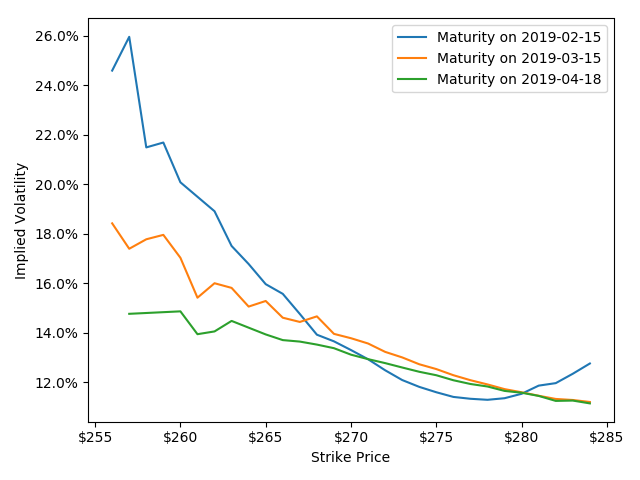
\includegraphics[width=.47\textwidth]{bin/vol_smile/SPY_Call_2DVolSmile.png} &
                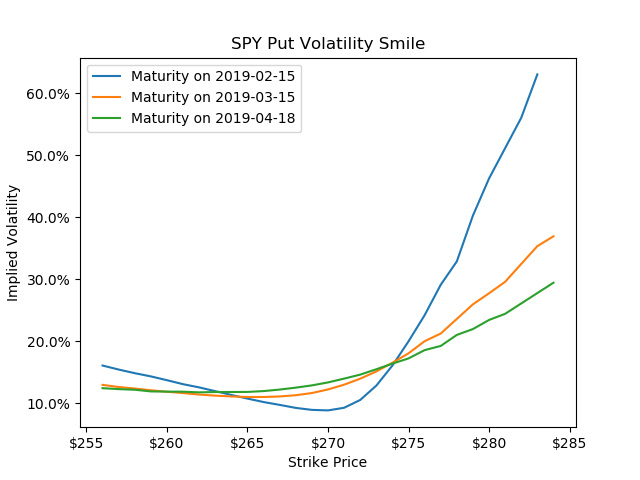
\includegraphics[width=.47\textwidth]{bin/vol_smile/SPY_Put_2DVolSmile.png} \\
                (a) SPY Call Option Volatility Smile &
                (b) SPY Put Option Volatility Smile \\
                \hline
                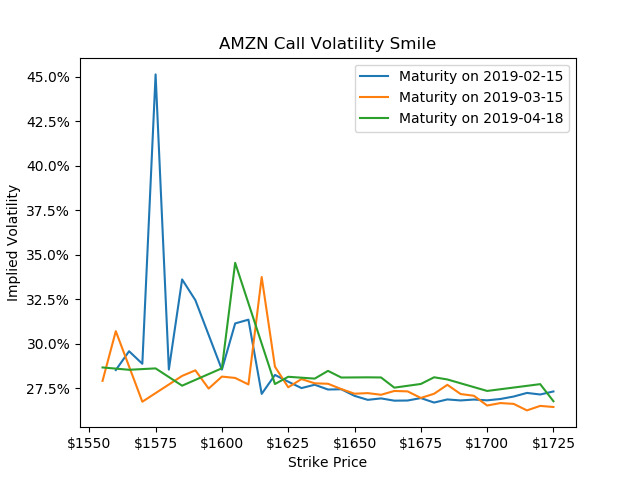
\includegraphics[width=.47\textwidth]{bin/vol_smile/AMZN_Call_2DVolSmile.png} &
                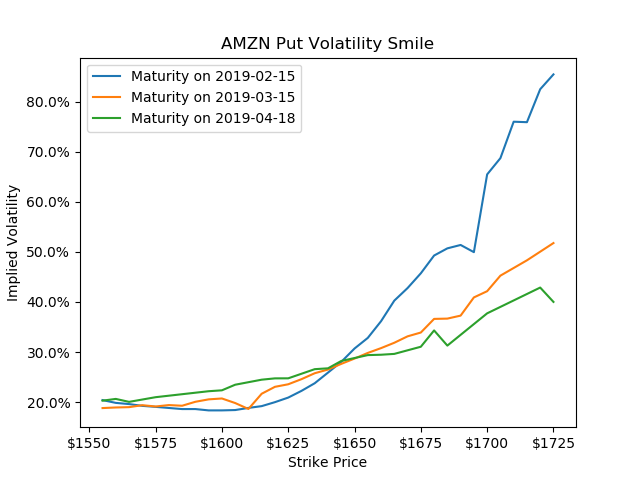
\includegraphics[width=.47\textwidth]{bin/vol_smile/AMZN_Put_2DVolSmile.png} \\
                (c) AMZN Call Option Volatility Smile &
                (d) AMZN Put Option Volatility Smile \\
                \hline
            \end{tabular}
            \label{fig:volatility_smiles}
            \caption{Volatility Smiles of call and put option chains on AMZN and SPY. Plots the relationship between the strike price and implied volatility for various maturities.}
        \end{figure}

        \subsubsection{Volatility Surface}

        \begin{figure}
            \begin{tabular}{|c|c|}
                \hline
                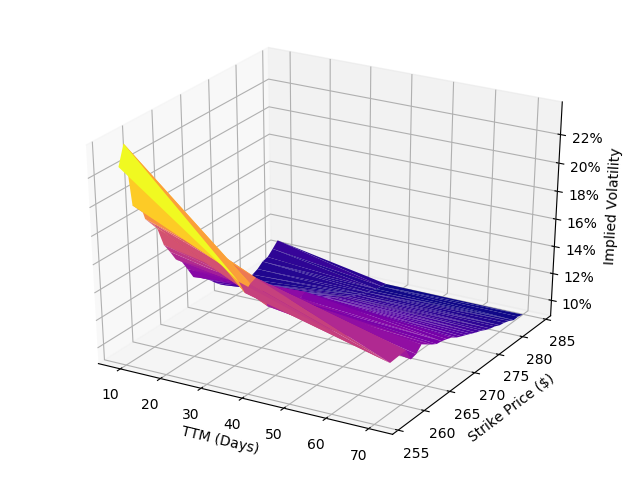
\includegraphics[width=.47\textwidth]{bin/vol_surface/SPY_Call_3DVolSurface.png} &
                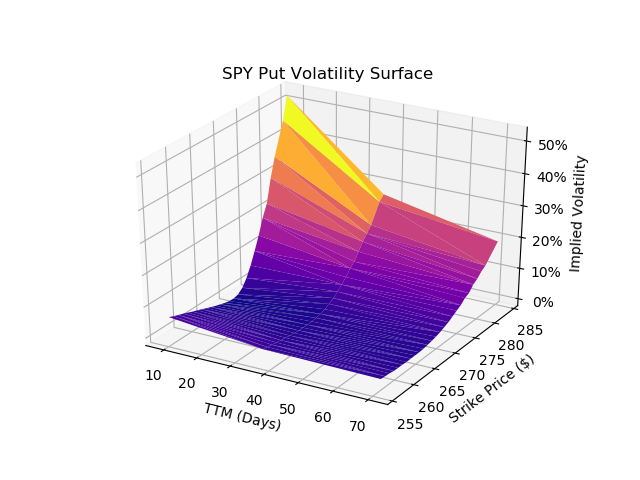
\includegraphics[width=.47\textwidth]{bin/vol_surface/SPY_Put_3DVolSurface.png} \\
                (a) SPY Call Option Volatility Surface &
                (b) SPY Put Option Volatility Surface \\
                \hline
                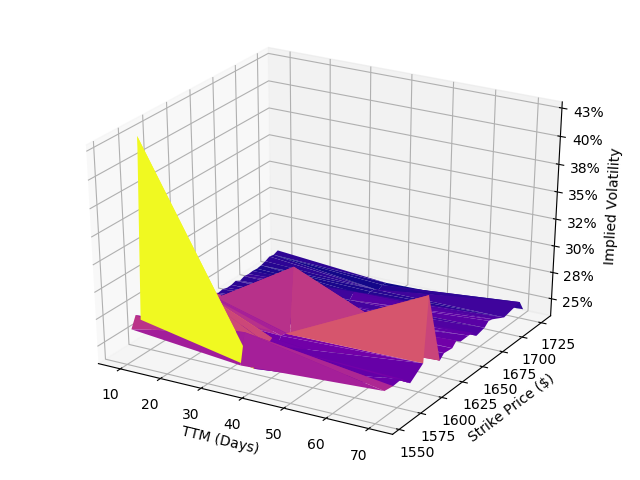
\includegraphics[width=.47\textwidth]{bin/vol_surface/AMZN_Call_3DVolSurface.png} &
                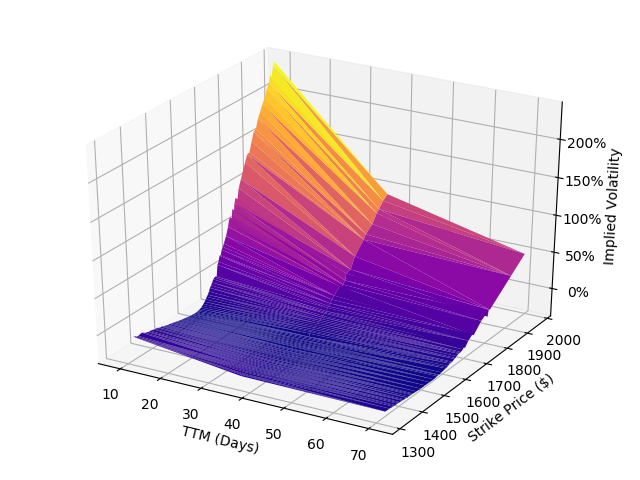
\includegraphics[width=.47\textwidth]{bin/vol_surface/AMZN_Put_3DVolSurface.png} \\
                (c) AMZN Call Option Volatility Surface &
                (d) AMZN Put Option Volatility Surface \\
                \hline
            \end{tabular}
            \label{fig:volatility_surfaces}
            \caption{Volatility Surfaces of call and put option chains on AMZN and SPY. Plots the relationship between the strike price, time to maturity, and the implied volatility.}
        \end{figure}


%==============================
% Section 3
%==============================
\newpage
\section{Numerical Integration}

    \subsection{Quadrature Methods}
    In this section, we implement the \textit{Trapezoidal Rule} and \textit{Simpson's Rule} quadrature methods.

    \begin{gather*}
        \text{Let data} = \boldsymbol{x} \\
        \text{Let $i^\text{th}$ element of $\boldsymbol{x}$} = x_i
    \end{gather*}

        \subsubsection{Trapezoidal Rule}

        \begin{gather*}
            \text{Let Trapezoidal rule approximation} = T_N(f) \\
            \Rightarrow T_N(f)
            = \sum_{i=1}^{N} \left[ \left( \frac{f(x_{i-1}) + f(x_i)}{2} \right) \times h \right] \\
            \Rightarrow h \times \sum_{i=1}^N \left[ \frac{f(x_{i-1}) + f(x_i)}{2} \right]
            = h \times \left( \frac{1}{2}f(x_0) + f(x_1) + \cdots + f(x_{N-1} + \frac{1}{2}f(x_N))\right) \\
            \therefore \, T_N(f) = hf(\boldsymbol{x}) - \frac{h}{2}(f(x_0) + f(x_N))
        \end{gather*}
        
        \lstinputlisting{fe621/numerical_integration/trapezoidal.py}

        \pagebreak[4]
        \subsubsection{Simpson's Rule}

        The following equation is derived in full in (\cite{Florescu2019}).

        \begin{gather*}
            \text{Let Simpson's rule approximation} = S_N(f) \\
            \Rightarrow S_N(f) \approx \frac{h}{6} \times \sum_{i=1}^N \left[ f(x_{i-1}) + 4f \left( \frac{x_{i-1} + x_i}{2} \right) + f(x_i) \right] \\
            = \frac{h}{6} \left( \sum_{i=1}^N [f(x_{i-1}) + f(x_i)] + 4 \times \sum_{i=1}^N \left[ f \left( \frac{x_{i-1} + x_i}{2} \right) \right] \right) \\
            \\
            \text{Note that $\left( \frac{x_{i-1} + x_i}{2} \right)$ is the midpoint between the points in $\boldsymbol{x}$.} \\
            \text{Let the above} = \boldsymbol{x_\text{mid}} \\
            \therefore \, S_N(f) \approx \frac{h}{6} \left( 2f(\boldsymbol{x}) - (f(x_0) + f(x_N)) + 4f(\boldsymbol{x}_\text{mid}) \right)
        \end{gather*}

        \lstinputlisting{fe621/numerical_integration/simpsons.py}
    
    \pagebreak[3]
    \subsection{Truncation Error Analysis}

    To examine the behavior of each of the quadrature methods described above, we approximate the integral of the following function:

    \begin{gather*}
        f(x) =
        \begin{cases}
            \frac{\sin{(x)}}{x}, & \quad \text{for} \, x \neq 0, \\
            1, & \quad \text{for} \, x = 0.
        \end{cases}
    \end{gather*}

    We parameterize the start and stop points of the quadrature methods with a variable $a$, such that ${\text{start} = -a}$ and ${\text{stop} = a}$. Furthermore, we define the number of segments with variable $N$.

    \begin{gather*}
        \text{Let approximation with parameters $a$ and $N$} = I_{N,a}
    \end{gather*}

    It is know analytically that the value of the integral $\int_\infty^\infty f(x) dx = \pi$. We evaluate the performance of each of the quadrature methods with various values of $a$ and $N$. Then, we compute the \textit{truncation error} of the approximation, defined as:

    \begin{gather*}
        \text{Truncation error for approximation with parameters $a$ and $N$} = \left| I_{N,a} - \pi \right|
    \end{gather*}

    \begin{table}[h]
        \centering
        \csvautotabular{bin/numerical_integration/trapezoidal_trunc_error.csv}
        \caption{Trapezoidal quadrature rule truncation error for varying values of $a$ and $N$.}
        \label{table:trapezoidal_trunc_error}
    \end{table}

    \begin{table}[h]
        \centering
        \csvautotabular{bin/numerical_integration/simpsons_trunc_error.csv}
        \caption{Simpsons quadrature rule truncation error for varying values of $a$ and $N$.}
        \label{table:simpsons_trunc_error}
    \end{table}

    Table~\ref{table:trapezoidal_trunc_error} and Table~\ref{table:simpsons_trunc_error} report the truncation error for the Trapezoidal and Simpson's quadrature rules, respectively. The script used to produce this table is reproduced in Appendix~\ref{appendix:q3:source:trunc_error}. Variations of $N$ and $a$ are explores in increasing powers of 10, with $a$ progressing from 100 to 1,000,000, and $N$ from 1,000 to 10,000,000.

    It is evident from Table~\ref{table:trapezoidal_trunc_error} that the Trapezoidal quadrature rule performs relatively well across all values of $a$, even at relatively low values of $N$. Compared to Simpson's quadrature rule truncation error (Table~\ref{table:simpsons_trunc_error}), the Trapezoidal quadrature rule also performs relatively better with larger values of $N$, and small values of $a$.
    
    A potential explanation of this may be the interpolating behavior of the Simpson's quadrature rule. The function $\frac{sin{(x)}}{x}$ is significantly more linear than quadratic in small intervals, and thus the quadratic interpolating behavior of the Simpson's quadrature rule is a poor approximation heuristic for the function with low values of $a$.

    Finally, it can be observed that both quadrature rule approximations converge commensurately as the values of $a$ and $N$ increase. However, it is clear that the Trapezoidal quadrature rule approximation converges at a faster rate than the Simpson's quadrature rule approximation with increasing values of $a$ and $N$.

%==============================
% References
%==============================

\newpage

\printbibliography


%==============================
% Appendix
%==============================

\newpage

\appendix % all sections after this are appendix sections

% Resetting input path
\lstinputpath{}

\section{Computed Implied Volatility} \label{appendix:q2:imp_vol}
        
    \subsection{SPY Option Chain} \label{appendix:q2:spy_vol}
        \csvreader[
            longtable=lcccl,
            table head=
                \toprule\bfseries Option Name &\bfseries Expiration Date &\bfseries Type &\bfseries Strike &\bfseries Implied Volatility \\ \midrule \endhead \bottomrule \endfoot,
            late after line=\\
        ]{bin/spy_data1_vol.csv}{1=\one, 2=\two, 3=\three, 4=\four, 5=\five}{\one & \two & \three & \four & \five}
    
    \subsection{AMZN Option Chain} \label{appendix:q2:amzn_vol}
        \csvreader[
            longtable=lcccl,
            table head=
                \toprule\bfseries Option Name &\bfseries Expiration Date &\bfseries Type &\bfseries Strike &\bfseries Implied Volatility \\ \midrule \endhead \bottomrule \endfoot,
            late after line=\\
        ]{bin/amzn_data1_vol.csv}{1=\one, 2=\two, 3=\three, 4=\four, 5=\five}{\one & \two & \three & \four & \five}


\newpage
\section{Solution Source Code} \label{appendix:source}

    \subsection{Question 1 Implementation}

        \subsubsection{Bloomberg Terminal Data Download} \label{appendix:source:q1:bloomberg}
            \lstinputlisting{question_solutions/question_1.R}
    
    \newpage
    \subsection{Question 2 Implementation}
        
        \subsubsection{Optimization Method Convergence Comparison} \label{appendix:source:q2:convergence}
            \lstinputlisting{question_solutions/question_2_convergence.py}

        \subsubsection{Implied Volatility Computation} \label{appendix:source:q2:imp_vol}
            \lstinputlisting{question_solutions/question_2_imp_vol.py}
        
        \subsubsection{Volatility Plots} \label{appendix:source:q2:vol_plots}
            \lstinputlisting{question_solutions/question_2_vol_plots.py}

    \newpage
    \subsection{Question 3 Implementation} \label{appendix:q3}
        
        \subsubsection{Truncation Error Analysis} \label{appendix:q3:source:trunc_error}
            \lstinputlisting{question_solutions/question_3_trunc_error.py}


%==============================
% Document End
%==============================

\end{document}
